\chapter{Arhitektura i dizajn sustava "Alpinity"}

Kako bi se ostvarile prethodno opisane funkcionalnosti, sustav je koncipiran pomoću klijent-poslužitelj arhitekture. Ova arhitektura omogućuje fleksibilnost u razvoju aplikacije i direktno omogućuje korištenje različitih platformi za razvoj klijentskog softvera. Sustav se sastoji od tri neovisne komponente: centralnog pozadinskog sustava (eng. \textit{Backend}), mobilne aplikacije za iOS kao primarni klijent te web aplikacije kao komplementarnog klijenta. 
Komunikacija između klijenata i pozadinskog sustava odvija se putem definiranog REST servisa. Pozadinski sustav automatski generira OpenAPI specifikaciju koja služi kao formalna dokumentacija koju klijenti mogu koristiti za generiranje potrebnih funkcionalnosti za poziv servisa. Time se osigurava konzistentnost funkcionalnosti te olakšava paralelni razvoj.

\begin{figure}[H]
    \centering
    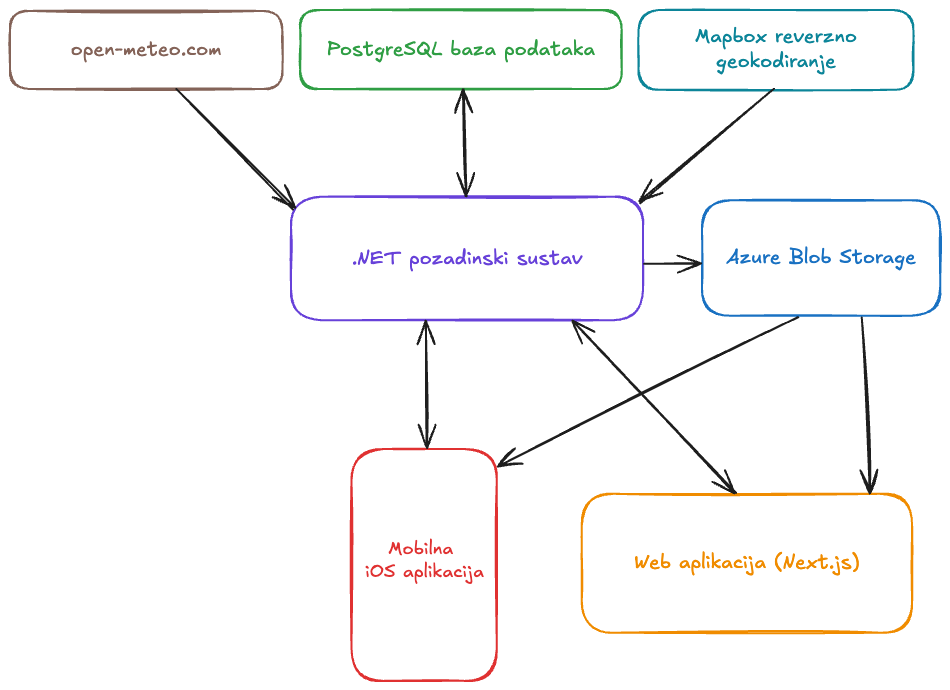
\includegraphics[width=0.9\textwidth]{images/arhitektura/general_arch.png}
    \caption{Makro arhitektura sustava}
    \label{fig:arhitektura}
\end{figure}

Slika~\ref{fig:arhitektura} prikazuje makro arhitekturu sustava te međusobne veze između komponenata. Mobilna i web aplikacija su neovisne komponente koje komuniciraju s pozadinskim sustavom putem REST servisa. Kada postoji neka slika, primjerice na detaljnom pregledu penjališta, pozadinski sustav šalje te slike u obliku poveznice na Azure Blog Storage servis. Također, web i mobilna aplikacije obije nemaju direktan pristup \textit{open-meteo} API-ju ni bazi podataka u obliku PostgreSQL baze podataka već se informacije agregiraju i šalju preko pozadinskog sustava.

\section{Pozadinski sustav (Backend)}

Pozadinski sustav predstavlja središnji dio cjelokupne arhitekture, odgovoran za svu poslovnu logiku, upravljanje podacima i komunikaciju s vanjskim servisima. Ključne odgovornosti pozadinskog sustava obuhvaćaju implementaciju RESTful API-ja za sve operacije, autentifikaciju i autorizaciju, te dohvaćanje i pohranu podataka iz relacijske baze podataka. Razvijen je korištenjem .NET platforme i ASP.NET core okvira, koji je odabran zbog visokih performansi i dobre podrške za razvoj modernih web servisa. Za organizaciju poslovne logike i smanjenje ovisnosti između unutarnjih komponenti pozadinskog sustava, sustav implementira Mediator uzorak (eng. \textit{Mediator pattern}). Ovaj pristup omogućuje da se zahtjevi s klijentskih aplikacija ponašaju kao neovisne poruke koje se zatim prosljeđuju odgovarajućim rukovateljima (eng. \textit{Handlers}), čime se postiže čišća arhitektura programskog koda. Pozadinski sustav podijeljen je u četri dijela.

\subsection{Sloj domene}

Sloj domene sadrži temeljnu poslovnu logiku i pravila koja su neovisna o bilo kojoj vanjskoj tehnologiji. Ovaj sloj nema ovisnosti o drugim slojevima u arhitekturi. Njegove ključne komponente su entiteti, koji predstavljaju objekte poslovne domene poput korisnika, penjališta, smjerova te objekte informacija vremenske prognoze i reverznog geokodiranja, definirajući njihovo stanje i ponašanje. Uz objekte domene, ovaj sloj sadrži i enumeracije koje predstavljaju moguće vrijednosti za određene objekte poput tipove penjačkih smjerova ili načine uspona.

\subsection{Aplikacijski sloj}

Aplikacijski sloj orkestrira korištenje domenskih objekata kako bi izvršio specifične korisničke slučajeve (eng. \textit {use cases}), djelujući kao posrednik između vanjskog svijeta i unutarnje poslovne logike. Za organizaciju, ovaj sloj implementira Mediator uzorak (engl. Mediator pattern). Svaki korisnički slučaj implementiran je kao trojka koji se sastoji od naredbe, što je poruka koja opisuje namjeru, validatora koji validira dobivenu naredbu te rukovatelja (engl. handler), klase koja prima poruku i izvršava potrebnu logiku. Ovaj sloj ovisi isključivo o sloju domene i definira logiku aplikacije bez znanja o tome kako će podaci biti prikazani ili pohranjeni.


\subsection{Infrastrukturni sloj}

Infrastrukturni sloj sadrži konkretne implementacije tehnologija koje su potrebne aplikaciji za rad. Ovaj sloj ovisi o aplikacijskom sloju kako bi implementirao njegova sučelja i sadrži sve što je promjenjivo i vanjsko. Ovdje se nalaze implementacije repozitorija koje koriste Entity Framework Core za komunikaciju s PostgreSQL bazom podataka. Također, ovaj sloj sadrži i integracije s vanjskim servisima: klijente za Azure Blob Storage za pohranu slika, open-meteo.com servis za vremensku prognozu i Mapbox servis za reverzno geokodiranje.

\subsection{Prezentacijski sloj}

Prezentacijski sloj je ulazna točka u pozadinski sustav, a u ovom slučaju to je ASP.NET Core Web API projekt. Njegova jedina odgovornost je primanje HTTP zahtjeva, prosljeđivanje odgovarajućih naredbi aplikacijskom sloju putem Mediator-a, te formatiranje rezultata u HTTP odgovore u JSON formatu. Ovaj sloj također automatski generira i OpenAPI specifikaciju, koja služi kao interaktivna dokumentacija API-ja i olakšava razvoj klijentskih aplikacija.


\subsection{Vanjski servisi}

Za pohranu slika, kao što su profilne slike korisnika i referentne slike penjačkih smjerova, koristi se Azure Blob Storage. Ovaj servis je odabran zbog pouzdanosti i lakoće integracije s pozadinskim sustavom. Kako bi se obogatile informacije penjališta koriste se dva vanjska servisa. Za dohvat detaljne vremenske prognoze penjališta koristi se open-meteo.com servis. Prednosti open-meteo servisa naspram drugih servisa za vremensku prognozu je mogućnost pregleda vremenske prognoze daleko u budućnosti, velike količine podataka koji se mogu dohvatiti te mogućnost izbora točno određenih podataka koji su potrebni. Za dohvat imena geografske lokacije iz GPS koordinata (reverzno geokodiranje) koristi se Mapbox servis. Mapbox servis je odabran jer je već korišten na web aplikaciji i nudi dobru podršku za reverzno geokodiranje.

\subsection{Model baze podataka}
Vidi sa mentoricom jel ovo previše.

\section{Mobilna aplikacija za iOS}

Mobilna aplikacija predstavlja primarni klijent sustava "Alpinity", posebice za korištenje na terenu. Razvijena je nativno za iOS platformu korištenjem SwiftUI okvira. SwiftUI je odabran kao moderno, deklarativno sučelje koje omogućuje razvoj kompleksnih korisničkih sučelja. Arhitektura aplikacije slijedi moderne principe razvoja za iOS, s jasnom podjelom odgovornosti između korisničkog sučelja, poslovne logike i komunikacije s pozadinskim sustavom. 

Za komunikaciju s pozadinskog sustava, aplikacija koristi swift-openapi-generator. Ovaj alat automatski generira Swift klijentski kod iz OpenAPI specifikacije, osiguravajući tipsku sigurnost i eliminirajući potrebu za ručnim pisanjem mrežnog sloja. Time se značajno ubrzava razvoj i smanjuje mogućnost pogrešaka. Za sigurno pohranjivanje korisničkog tokena za autentifikaciju i održavanje sesije, koristi se biblioteka KeychainAccess, koja pruža jednostavno i sigurno sučelje za rad s iOS Keychain servisom. Za prikaz interaktivnih geografskih karata, aplikacija se oslanja na nativni Apple Maps servis. Finalno, za spremanje podataka za izvanmrežni način rada, koristi se nativni SwiftData okvir.

\subsection{Implementacija prepoznavanja smjerova pomoću OpenCV}

Prepoznavanje penjačkih smjerova pomoću proširene stvarnosti implementirano je korištenjem biblioteke OpenCV. Svi računski intezivni zadaci računalnog vida izvršavaju se izravno na korisnikovom uređaju.

Da bi se postigao rad u stvarnom vremenu, ključno je efikasno upravljati kardovima koji dolaze s kamere. Aplikacija koristi moderni pristup temeljen na asinkronim tokovima podataka (eng. \textit{asynchronous streams}). Kamera kontinuirano emitira kadrove, no obrada svakog pojedinog kadra bila bi računski preskupa i dovela bi do zagušenja sustava. Zbog toga je implementiran mehanizam za prorjeđivanje kadrova (eng. \textit{frame dropping}). 
Koristi se \textit{AsyncStream} s politikom \textit{bufferingOldest(1)}, što znači da se u svakom trenutku čuva samo najstariji neobrađeni kadar. Ovaj pristup osigurava da sustav za obradu, time i korisnikov uređaj, nije preopterećen, čak i ako obrada jednog kadra traje duže od intervala između dva kadra.

Svaki kadar koji se propusti na obradu prolazi nizom operacija definiranih OpenCV funkcijama, sljedeći teorijske korake opisane u 3. poglavlju. Prvo se, radi optimizacije, smanjuje rezolucija ulaznog kadra ovisno o jačini prepoznavanja koje je korisnik postavio. Na tako pripremljenoj slici primjenjuje se SIFT algoritam pozivom metode \textit{sift.detectAndCompute}, koja ekstrahira ključne točke i njihove deskriptore. 
Nakon toga slijedi uparivanje s referentnim deskriptorima korištenjem \textit{flannMatcher.knnMatch} metode, a rezultati se filtriraju primjenom Loweovog testa omjera. Iz skupa preostalih dobrih podudarnosti, pozivom funkcije \textit{findHomography} s RANSAC metodom, izračunava se robusna matrica homografije.

Rezultat ovog procesa obrade je izobličena referentna slika linije penjačkog smjera s transparentnom pozadinom, dobivena primjenom izračunate homografije na originalnu sliku linije pomoću \textit{warpPerspective} funkcije. Ovakav izlaz omogućuje potpunu nezavisnost kadrova kamere i rezultata obrade kadrova, što omogućuje prikazivanje kadrova kamere bez ikakvih ograničenja, a rezultat se samo nadodaje na kadar kada se obradi. 
Ta slika ostaje spremljena i nacrtana preko novih kadrova dok se ne pojavi nova izobličena referentna slika. Ovakva organizacija procesa obrade omogućuje fluidno korisničko iskustvo sa nedostatkom što izobličene linije penjačkih smjerova kasne naspram kadrova. Unatoč ovom nedostatku, značajnija je prednost što jačina prepoznavanja može biti mnogo veća nego da se kadar kamere i izobličena referentna slika linije penjačkog smjera prikazuju sinkrono.

\subsection{Kreiranje referentne slike penjačkog smjera}

Aplikacija također sadrži i funkcionalnost za kreiranje referentnih podataka. Kada korisnik korištenjem kamere napravi sliku i na njoj iscrta putanju penjačkog smjera smjera, aplikacija poziva metodu koja prima niz koordinata koje predstavljaju putanju penjačkog smjera i referentnu sliku. Prvo stvara praznu, prozirnu matricu istih dimenzija kao i referentna slika. Dimenzija referentnih slika moraju biti identične kako bi algoritam mogao zamjeniti sliku s linijom prilikom procesa transformacije perspektive. Zatim, koristeći \textit{OpenCV} metodu \textit{polylines}, iscrtava liniju na tu matricu. Zanimljivo je da se linija iscrtava dva puta, prvo deblja crna linija, a zatim preko nje tanja crvena linija, čime se postiže vizualni efekt obruba. Rezultirajuća matrica se pretvara u sliku s linijom te se zatim šalje na poslužitelj i sprema na Azure Blob Storage i u bazu podataka kao poveznicu na Azure Blob Storage.


\section{Web aplikacija}

Uz mobilnu aplikaciju, sustav "Alpinity" uključuje i web aplikaciju. Njena temeljna svrha je pružiti korisnicima sučelje za pregled i upravljanje podacima na većim ekranima ili na android uređajima. Web aplikacija nudi sve funkcionalnosti dostupne na mobilnoj aplikaciji, s iznimkom onih koje su vezane uz hardver mobilnog uređaja, poput prepoznavanja smjerova pomoću kamere.

Aplikacija je razvijena korištenjem Next.js okvira, koji se temelji na React biblioteci. Next.js je odabran zbog svojih naprednih mogućnosti koje osiguravaju visoke performanse. Korištenjem tehnika poput renderiranja na poslužitelju postiže se iznimno brzo učitavanje sadržaja.

Korisničko sučelje je izgrađeno korištenjem biblioteke komponenata shadcn/ui. Ona omogućuje brzu i konzistentnu izradu vizualno dopadljivog i pristupačnog sučelja, temeljenog na prilagodljivim i višekratno iskoristivim komponentama. Za prikaz interaktivnih geografskih karata, web aplikacija koristi Mapbox platformu.

Komunikacija s pozadinskim sustavom riješena je na konzistentan i tipski siguran način. Korištenjem alata hey-api/openapi-ts, klijentski kod za pozivanje pozadinskog sustava automatski se generira iz OpenAPI specifikacije koju generira sam pozadinski sustav. Ovaj pristup, analogan onome korištenom u mobilnoj aplikaciji, osigurava da su klijent i poslužitelj uvijek usklađeni, smanjuje mogućnost pogrešaka i značajno ubrzava proces razvoja.